\chapter{La genesi} \label{cap:papert}

\section{La paura della matematica}

Perché la motivazione fondamentale della genesi di Logo sta tutta nella questione, tutt'ora irrisolta, dell'insegnamento della matematica. Il linguaggio Logo è stato ideato da Papert proprio per cercare di risolvere questo annoso problema per il quale aveva coniato anche un preciso nome, \textit{Mathofobia}, per descrivere la diffusa antipatia verso questa materia. L'interesse di Papert per la questione ha accompagnato tutta la sua vita lavorativa, che si è distesa nella seconda metà del 900. Il suo contributo è stato eccezionale, sia sotto il profilo dell'elaborazione teorica dal punto di vista pedagogico, che della creatività che lo ha condotto a concepire appositamente un linguaggio per avvicinare i ragazzi alla matematica. La profonda competenza, sia nelle questioni matematico-informatiche che in quelle pedagogiche, rende la sua opera unica e spiega la rara capacità di proporre soluzioni concrete. 

La sensazione è che non molto sia cambiato, dagli anni '80 ad ora, almeno in media\footnote{Affermazione che nasconde un mondo di perplessità. Cosa è cambiato? Forse proprio ciò che una “media” non esprime. La scuola cui si riferiva Papert è probabilmente più affine a quella che ha frequentato il sottoscritto (I elementare nel 1960). Allora probabilmente il panorama era più uniforme. “La lo picchi se non capisce perché gliè zuccone!” raccomandò la mamma di un mio compagno di classe alla maestra. I genitori erano alleati di quel sistema scolastico, in una visione formativa che poteva essere coercitiva e punitiva, ma che attraversava tutti i generi di scuole e tutti gli strati sociali. Non c'erano “genitori coach” o “genitori sindacalisti”. Nelle famiglie si lavorava duramente, nelle scuole si faticava. Non c'era ancora il “tempo libero”. La scuola era più brutale, forse iniqua, la pedagogia semplice, ma il panorama era più nitido. Almeno nella provincia rurale degli anni '60 in cui ho vissuto. Ora domina la complessità. Le categorie si intersecano. I dibattiti esplodono, amplificati dai media, a livello microscopico (gruppi di genitori in Wathsapp o Facebook) e a livello macroscopico (stampa, televisione ecc.). Le esperienze personali sono schizofreniche: i miei contatti con il mondo dell'insegnamento rappresentano un quadro affascinante di impegno, studio e sperimentazione; ma le storie private e le narrazioni dei conoscenti sono popolate di pratiche didattiche obsolete e superficiali. La variabilità è allucinante. Dove sta la media? Francamente non sono in grado di valutarlo ma la dispersione è sicuramente molto più ampia di un tempo. A complicare il quadro ci sono le indagini internazionali, paludate di rigore scientifico ma che poi si possono rivelare speratamente fatue. Per alcuni anni è brillata la stella polare della Finlandia nel cielo delle valutazioni PISA dell'OCSE, in particolare per la matematica. Poi emergono una serie di denunce di accademici finlandesi che documentano un crollo delle competenze matematiche: sembra che gli studenti finlandesi siano diventati bravi nei test matematici PISA ma che siano peggiorati in matematica! Leggendo il post di Giorgio Israel “Il bluff della matematica finlandese” (http://gisrael.blogspot.it/2011/05/il-bluff-della-matematica-finlandese.html), che riassume tali denunce, si scopre che i modelli di apprendimento sono banalmente utilitaristici e anche ben lontani dalle idee di Papert che riportiamo qui. Dove sarà la verità? Insomma la confusione regna sovrana e viene seriamente da domandarsi se non ci si debba rassegnare a considerarla inevitabile normalità.}; che la motivazione iniziale, centrata su una seria e difficile rivisitazione del modo di introdurre i giovani alla matematica, sia finita diluita oggi nel calderone del “coding”, nella forma di una sorta di paese dei balocchi, superficialmente entusiasmante per taluni, oggetto di derisione per altri; che il messaggio di Papert, per certi versi estremo e provocatorio, senz'altro da decodificare rispetto ad un'epoca diversa, venga frainteso; che il tutto sia vanificato in sostanza dal fallimento di Logo, rimasto confinato in una minoranza di circoli sperimentali, senza avere rivoluzionato nulla, contrariamente a quelle che sembravano le legittime aspettative di Papert; che invocare la magia della matematica per introdurre i giovani in un dominio comunemente considerato “freddo”, sia un sogno che alla fin fine può concepire solo un matematico, magari un po' idealista, e quindi che solo un'arida via può svelare quella magia, e solo ai pochi in grado di percorrerla, per un motivo o per un altro, e che non possa essere infine altro che così – una cosa che io non voglio pensare ma la paura che sia un po' vera m'è venuta rileggendo \textit{Mindstorms}.

Logo fallito abbiamo detto. Ha fallito nelle intenzioni iniziali di Papert. Non è diffuso nelle scuole e non è adottato come un modo standard per sostenere l'apprendimento della matematica e delle scienze. Ma non ha fallito nel senso di non aver lasciato traccia, al contrario. Ci sono molte versioni del logo in tutto il mondo, alcune delle quali sono diventate importanti strumenti di indagine educativa, ad esempio nel campo della simulazione di sistemi biologici complessi. Ed è sempre da Logo che ha preso spunto il vasto mondo dei linguaggi visivi a blocchi, primo fra tutti Scratch. Logo e Scratch non sono in opposizione. In un certo senso, Scratch deriva da Logo e "contiene" molte delle sue funzionalità. Molte delle cose che puoi fare in Logo possono essere fatte anche in Scratch. Ma Scratch è molto più orientato alla costruzione "del tuo videogioco" o allo storytelling. Il problema, tuttavia, è che questa gamma più ampia di possibilità, in un contesto scolastico caratterizzato da un basso livello di istruzione tecnologica, ha finito per disperdere le intenzioni educative originali di Logo. Una delle intenzioni di questo manuale è quella di recuperare l'originale "sapore matematico" della pratica del \textit{coding} a scuola. Nella prossima sezione commentiamo quella che Papert ha chiamato \textit{mathophobia}, una sorta di malattia che Logo era destinato a combattere. 

\section{\textit{\textit{Mathophobia}: The Fear for Learning}}

Seymour Papert ha scelto di intitolare il secondo capitolo di Mindstorms "Mathophobia: The Fear for Learning". Il suo punto di partenza è la divisione schizofrenica tra scienze umane e scientifiche, una divisione che è profondamente radicata nel linguaggio, nella visione del mondo, nell'organizzazione sociale e nel sistema educativo. Una divisione che negli ultimi 30-40 anni di deriva neoliberista, si è ulteriormente ampliata. Ad esempio, nelle università, a partire dagli anni '80, gli accademici si battono per ottenere i finanziamenti necessari per le loro ricerche. Purtroppo, l'altra faccia della medaglia è che quasi nessuno si preoccupa di insegnare, o molto poco. La carriera di un professore non dipende dalla qualità del suo insegnamento, ma quasi solo dalla quantità della sua produzione scientifica. Le conseguenze sono pessime. Gli accademici tendono a trasformarsi in manager quando fanno ricerca e in funzionari pubblici quando insegnano: imprenditori dinamici da un lato e (forti) conservatori dall'altro. In questo modo, anche nelle scienze umane si assiste a una deriva tecnica del ruolo accademico. La missione dell'insegnamento, che in un certo senso è il "lato umanistico" del lavoro, si riduce a una sorta di Cenerentola. Così, la dicotomizzazione tra scientifico e umanistico è ancora più forte e sbilanciata.

La questione non è quella di un equilibrio adeguato, bensì di spezzare la linea di demarcazione tra le due culture. Papert guardò il computer come una forza per attenuare la distinzione. La pratica del \textit{coding} è stata pensata come un modo per introdurre una matematica più umanistica e per sfruttare elementi di pensiero scientifico nelle scienze umane. È in questo contesto che Papert ha parlato di una \textit{Mathland}, dove la matematica costituirebbe un vocabolario naturale, con l'idea che potremmo cambiare non solo il modo in cui insegniamo la matematica, ma anche il modo in cui la nostra cultura concepisce la conoscenza e l'apprendimento.

Papert sostiene che le sue argomentazioni non si limitano all'apprendimento della matematica, ma riguardano anche l'atteggiamento nei confronti dell'apprendimento in generale. La parola \textit{mathphobia} suggerisce due associazioni. Una è il diffuso timore per la matematica. L'altra deriva dalla radice "math", che in greco antico significa apprendimento in senso generale. Così, se i bambini iniziano ad essere abili studenti spontanei, in seguito "imparano" la paura di imparare qualsiasi cosa e non solo la matematica. Ironia della sorte, sembra che più si studia, più si ha paura di imparare.

I bambini imparano migliaia di parole prima di entrare in prima elementare. Meno evidente per molte persone è il fatto che i bambini imparano una grande quantità di matematica pure. Tra queste conoscenze prescolare ci sono per esempio nozioni come la conservazione del volume di liquidi in recipienti di forma diversa, o l'indipendenza del numero totale di oggetti dall'ordine con il quale sono stati contati. Papert ha chiamato questo 

\begin{quote}
apprendimento Piagetiano, un processo di apprendimento che ha molte caratteristiche che le scuole dovrebbero invidiare: è efficace (tutti i bambini ci arrivano), è economico (sembra non richiedere né insegnanti né uno sviluppo del curriculum), ed è umano (i bambini sembrano farlo in uno spirito spensierato, senza esplicita ricompensa esterna e punizione).
\end{quote}.  

Infatti, le pratiche dell'insegnamento della matematica sottovalutano in larga misura l'apprendimento piagetiano, imponendo conoscenze formali che risultano per lo più dissociate dalle precedenti nozioni spontanee. Le conseguenze per i futuri adulti sono pesanti. La perdita dell'atteggiamento positivo del bambino nei confronti dell'apprendimento è un fenomeno molto comune nell'età adulta e non riguarda solo la matematica:

\begin{quote}
La deficienza diventa identità: "Non posso imparare il francese, non ho orecchio per le lingue"; "Non potrei mai essere un uomo d'affari, non ho una testa per le cifre".
\end{quote}.  

Circa l'80\% dei miei studenti di scuola primaria si dichiara "distante dalla matematica". Molti sostengono di avere difficoltà anche con le tecnologie, nonostante si supponga che siano "nativi digitali".

L'idea che ci siano persone intelligenti e stupide ai fini di una data attività è diffusa. È estremamente difficile sradicare i pregiudizi sui propri atteggiamenti. Il punto è che le convinzioni accettate circa l'attitudine matematica non sono dimostrabili. Per rafforzare il concetto, Papert ha riformulato l'argomento come segue \cite{Papert} (p. 43):

\begin{quote}
Immaginiamo di far disegnare ai bambini per un'ora al giorno passi di danza sulla carta e di far sostenere loro un esame su tali “questioni di danza” prima di lasciarli ballare veramente. Non dovremmo in tal caso aspettarci un mondo pieno di “danzofobi”? E non concluderemmo che coloro che ce la fanno a raggiungere la sala da ballo sono i più dotati per la danza? Io credo che sia altrettanto ingiustificato trarre conclusioni  sulle doti matematiche in base allo scarso entusiasmo dei bambini per passare centinaia di ore a fare somme.
\end{quote}.

Spesso è la scuola che costruisce le attitudini:

\begin{quote}
Consideriamo il caso di un bambino  che ho seguito durante i suoi ottavo e nono anni di età. Jim era un bambino molto loquace ma matofobico appartenente ad una famiglia di professionisti. La sua passione per le parole e il piacere di parlare si erano manifestate molto prima di andare a scuola. La matofobia era invece comparsa a scuola. La mia teoria è che essa sia stata una diretta conseguenza della sua precocità verbale. Dai genitori avevo appreso che Jim aveva presto sviluppato l'abitudine di commentare a voce alta qualsiasi cosa facesse. Un'abitudine che non aveva causato particolari problemi con i genitori o presso la scuola dell'infanzia. I problemi sono sorti affrontando l'aritmetica. A quel punto aveva già imparato a tenere sotto controllo la sua abitudine ma io sospetto che lui non avesse cessato di commentare le proprie azioni, seppur interiormente. Durante le ore di matematica si trovava in imbarazzo: semplicemente non riusciva a commentare l'attività di fare somme. Gli mancava il vocabolario (come manca alla maggior parte di noi) e non vedeva la motivazione. Questa frustrazione si tramutò in odio per la matematica, la conseguenza del quale fu una valutazione di scarsa attitudine per la materia. 

Per me fu una storia commovente. Credo che molto spesso quella che appare una debolezza intellettuale sia espressione, come nel caso di Jim, di quella che in realtà è una particolare capacità. È non è solo la capacità verbale, chiunque osservi con attenzione i bambini nota processi simili: per esempio un bambino che prediliga l'ordine logico può avere problemi con la sillabazione dell'inglese e magari finire col detestare la scrittura.
\end{quote}.

L'idea di Papert era che si possono usare i computer come veicoli per risolvere situazioni come quella di Jim o quella di bambini che, all'opposto, amano la logica, ma presentano problemi di tipo dislessico. Entrambi i casi sono vittime della netta separazione della nostra cultura tra "il verbale" e "il matematico". Egli immagina una sorta \textit{Mathland} dove l'amore di Jim per la lingua e la sua abilità potrebbero essere mobilitati per realizzare l'apprendimento matematico formale, invece di contrastarlo, mentre per l'altro tipo di bambini, l'amore per la logica potrebbe nutrire l'interesse per la linguistica. I metodi di insegnamento prevalenti danno agli studenti di matematica possibilità limitate di reperire un senso in ciò che stanno imparando. Di conseguenza, i bambini sono costretti a seguire il modello peggiore per l'apprendimento della matematica, che è l'apprendimento mnemonico, dove l'oggetto di studio sembra non avere senso. È quello che Papert chiamava un modello di apprendimento \textit{dissociato}.

\begin{quote}
Nel corso di uno studio di un anno, in una classe II di scuola  media di I grado di livello medio, una delle attività era quella che gli studenti chiamavano “\textit{computer} \textit{poetry}”. L'attività consisteva nell'usare il computer per comporre frasi: loro inserivano una struttura sintattica che il computer popolava di parole in maniera casuale. Il risultato è una sorta di poesia concreta tipo quella illustrata qui sotto\footnote{[NdR] Ho lasciato la versione originale, mi pare inutile “tradurre” un pezzo simile, ai fini della comprensione del concetto. Ho riportato questo esempio perché verrà ripreso, in altra forma, in uno degli esempi più avanzati di impiego di Logo. É interessante che ciò che negli anni 70 richiedeva un potente computer e uno staff di ricerca avanzato ora si possa fare con una semplice implementazione di Logo in un PC.}:
\end{quote}

\begin{quote}
INSANE RETARD MAKES BECAUSE SWEET SNOOPY SCREAMS\\
SEXY GIRL LOVES THATS WHY THE SEXY LADY HATES\\
UGLY MAN LOVES BECAUSE UGLY DOG HATES\\
MAD WOLF HATES BECAUSE INSANE WOLF SKIPS\\
SEXY RETARD SCREAMS THATS WHY THE SEXY RETARD\\
THIN SNOOPY RUNS BECAUSE FAT WOLF HOPS\\
SWEET FOGINY SKIPS A FAT LADY RUNS\\
\end{quote}

\begin{quote}
Un'allieva di tredici anni, Jenny, aveva commosso lo staff del progetto chiedendo il primo giorno: “Perché avete scelto noi? Noi non siamo i cervelloni. (“\textit{Why were we chosen for this? We're not the brains.}”. Lo studio prevedeva proprio di lavorare con una classe di livello “medio”. Un giorno Jenny entrò tutta eccitata. Aveva fatto una scoperta: “Ora ho capito perché ci  sono i sostantivi e i verbi.” Già da vari anni Jenny aveva fatto esercizi grammaticali, ma non aveva mai capito le differenze fra sostantivi, verbi e avverbi. Ma ora era chiaro che le sue difficoltà non dipendevano dall'incapacità di lavorare con categorie logiche. Il problema era un altro. Lei non aveva semplicemente compreso la finalità della fatica. Non era stata in grado di afferrare il senso della grammatica perché non vedeva a cosa servisse. E quando aveva chiesto a cosa serviva, la spiegazione dell'insegnante le era parsa manifestamente disonesta: “La grammatica ti serve a parlare meglio.”

Infatti, per recuperare la connessione fra l'apprendimento della grammatica e il miglioramento della lingua parlata occorre una visione più ampia del complesso procedimento di apprendimento di una lingua, che Jenny non poteva avere all'età in cui era entrata in contatto con la grammatica. Certamente lei non poteva vedere in che modo la grammatica potesse aiutarla a parlare meglio, né pensava di avere necessità di essere aiutata. Di conseguenza aveva sviluppato un sentimento di rancore per la grammatica. E, come succede alla maggior parte di noi, il rancore garantisce fallimento. Ma quando si è trovata nella condizione di far comporre frasi al computer, è successo qualcosa di interessante, trovandosi nella condizione di dover classificare le parole in categorie non perché qualcuno le avesse chiesto di farlo ma perché ne aveva bisogno. Per “insegnare” al suo computer come comporre serie di parole in maniera che sembrassero frasi compiute occorreva “insegnargli” a scegliere parole appartenenti alle categorie giuste. Ciò che lei aveva imparato sulla grammatica tramite l'esperienza con una  macchina non aveva niente di meccanico né di routinario. Il suo era stato un apprendimento profondo e significativo. Jenny aveva fatto più che imparare le definizioni per una particolare classe grammaticale. Aveva capito l'idea generale che le parole (come le cose) possono essere collocate in gruppi o insiemi diversi, e che fare questo può essere utile. Non aveva solo “capito” la grammatica ma aveva cambiato il suo atteggiamento nei suoi confronti. Era “sua”, e nel corso dell'anno, altri casi simili l'aiutarono rivedere la propria immagine. Cambiarono anche i suoi risultati; i suoi voti, prima medio-bassi, divennero massimi per il resto degli anni scolastici. Imparò che anche  lei poteva essere “un cervellone”, dopo tutto.
\end{quote}

Papert è perentorio: spesso i bambini non riescono a capire a cosa servano realmente matematica e grammatica perché percepiscono quelle degli adulti come spiegazioni volutamente ambigue.

\begin{quote}
È naturale come matematica e grammatica non vengano capite dai bambini quando non sono capite da chi sta loro intorno e come, affinché la comprendano, occorra qualcosa di più di un insegnante che dica la cosa giusta o disegni il diagramma giusto alla lavagna. Ho chiesto a molti insegnanti e genitori cosa pensassero della matematica e perché fosse importante impararla. Pochi di loro hanno espresso una visione sufficientemente coerente da giustificare l'impiego di varie migliaia di ore della vita di un bambino per impararla, e questo i bambini lo sentono. Quando un insegnante spiega a uno studente che tutte quelle ore di aritmetica servono a essere in grado di controllare il resto al supermercato, questo non viene semplicemente creduto. I bambini interpretano tali “motivazioni” come un ulteriore esempio di malafede da parte degli adulti. Lo stesso effetto si manifesta dicendo ai bambini che la matematica scolastica è “divertente”, quando è loro chiaro che gli insegnanti che si esprimono così per divertirsi fanno tutt'altre cose. Ne aiuta molto spiegare che la matematica serve per diventare scienziati poiché la maggior parte di loro non prevede una cosa del genere.  La maggior parte dei bambini si rende conto che l'insegnante non ama la matematica più di quanto la amino loro e che la ragione per cui va fatta è semplicemente perché lo prevede il curricolo. Tutto ciò erode la fiducia dei bambini nel mondo degli adulti e nel processo di educazione. \textit{E io penso che introduca un elemento di profonda disonestà nella relazione educativa}\footnote{[NdR] Corsivo dell'autore.}.
\end{quote}

È importante tenere presente la differenza tra la matematica - un vasto campo di indagine la cui bellezza è raramente sospettata dalla maggior parte dei non addetti ai lavori - e la \textit{matematica scolastica}. Quest'ultima è una sorta di costruzione sociale, cioè un insieme di argomenti matematici determinati da una successione di circostanze specifiche. Un processo che non garantisce, \textit{per se}, il raggiungimento di un risultato ottimale. Ricorda la storia del layout della tastiera noto con la sigla QWERTY, che rappresenta i primi cinque tasti delle righe superiori. Questo accordo non ha una spiegazione razionale, ma solo storica. Fu introdotto perché i tasti delle prime macchine da scrivere tendevano ad incepparsi. Furono disposti così per ridurre le collisioni, separando i tasti che si susseguivano più frequentemente. La tecnologia delle macchine da scrivere migliorò rapidamente e in pochi anni il problema dell'inceppamento non fu più un problema ma la disposizione QWERTY rimase tal quale. A questo punto troppe persone conoscevano il layout QWERTY e la produzione di macchine da scrivere era troppo lontana per fare un passo indietro nella riprogettazione di un layout più razionale, ad esempio raggruppando i tasti più usati. 

La questione della tastiera QWERTY è un buon esempio di come le abitudini consolidate non rappresentino necessariamente la scelta migliore. Anche la matematica scolastica si è formata in un contesto storico diverso. Allo stesso modo questa idea di matematica si è consolidata profondamente e, ancora oggi, per la maggior parte delle persone è inconcepibile che la matematica possa essere anche qualcos'altro. Ricordo un noto professore di analisi matematica che, all'inizio del primo anno del corso di laurea in matematica, esortava i suoi studenti a dimenticare ciò che avevano imparato al liceo, poiché la matematica era un'altra cosa. 

La geometria della tartaruga è stata concepita per adattarsi ai bambini e, prima di tutto, per essere "appropriabile". Potremmo descrivere questo concetto attraverso alcuni principi. In primo luogo, il principio di continuità: le nuove conoscenze matematiche devono essere in continuità con quelle esistenti, quelle che i bambini hanno prima di andare a scuola. Poi il principio di potenza: la nuova conoscenza deve permettere agli studenti di realizzare progetti personali significativi, che non potrebbero essere realizzati senza di essa. Infine, il principio della risonanza culturale: i nuovi concetti devono avere un senso per i bambini nel loro contesto sociale; paradossalmente, anche nel contesto sociale degli adulti: non dobbiamo infliggere ai bambini qualcosa che non abbiamo compreso a fondo e, purtroppo, spesso con la matematica scolastica è proprio così. 

Tradotto con www.DeepL.com/Translator

Tradotto con www.DeepL.com/Translator



Tradotto con www.DeepL.com/Translator

Tradotto con www.DeepL.com/Translator


Tradotto con www.DeepL.com/Translator


%%%%%%%%%%%%%%%%%%%%%%%%%%%%%%%%%%%%%%%%%%%%

Platone sulla sua porta aveva scritto: “Che entrino solo i geometri”. I tempi sono cambiati. La maggior parte di coloro che cercano di entrare nel mondo intellettuale di Platone non conoscono la matematica né percepiscono la minima contraddizione con la sua prescrizione. La schizofrenica suddivisione che la nostra cultura traccia fra le discipline umanistiche e quelle scientifiche supporta il loro senso di sicurezza. Platone era un filosofo, e la filosofia è una materia umanistica tanto sicuramente quanto la matematica una scientifica.

Questa grande divisione è radicata nel nostro linguaggio, nella nostra visione del mondo, nell'organizzazione sociale, nel sistema educativo e, più recentemente, anche nelle teorie neurofisiologiche. È una divisione che si auto-perpetua: più la cultura è divisa, più ciascuna parte rinforza la separazione nella propria crescita.

Ho già suggerito come il computer possa costituire una forza che serva ad abbattere la divisione fra le “due culture”. So che l'umanista può ritenere discutibile che una tecnologia possa influenzare la propria opinione su quale tipo di conoscenza sia rilevante nell'insegnamento. Non meno minacciosa appare allo scienziato la diluizione del rigore causata dall'invasione di pensiero umanistico “annacquato”. Ciò nonostante io penso che con la tecnologia si possano gettare i semi di un'epistemologia culturale meno dissociata. 

La condizione della matematica nella cultura contemporanea presenta i sintomi più acuti di tale dissociazione. L'emergenza di una matematica “umanistica”, che non sia percepita in maniera separata dallo studio dell'uomo e delle discipline umanistiche, potrebbe essere il segno di un mutamento di prospettiva. In questo libro io cercherò di mostrare come un computer possa essere utilizzato per condurre i bambini in una relazione più umanistica e anche più umana con la matematica. Per fare questo dovrò andare oltre la matematica. Dovrò sviluppare una nuova prospettiva del processo di apprendimento medesimo. 

Non è raro che adulti intelligenti si riducano ad essere osservatori passivi della propria incompetenza in tutto ciò che non sia la matematica più rudimentale. E possono subire le conseguenze di una simile paralisi intellettuale anche nella ricerca di un lavoro. Ma le conseguenze secondarie, indirette, sono ancora più gravi. Una delle lezioni principali imparate dalla maggior parte delle persone nelle ore di matematica è una consapevolezza delle proprie rigide limitazioni. Costoro si formano un'idea balcanizzata della conoscenza umana che finiscono col percepire come un collage di territori separati da ferree cortine impenetrabili. Io non metto in discussione la sovranità dei territori intellettuali ma le restrizioni imposte alla libera circolazione fra questi. Non voglio ridurre la matematica alla letteratura o la letteratura alla matematica. Ma voglio argomentare come le rispettive mentalità non siano così separate come viene generalmente supposto. E per fare questo, mi servo di un'immagine, ovvero di una \textit{Mathland}  – dove la matematica sia un vocabolario naturale – al fine di sviluppare l'idea che con la presenza del computer le culture umanistica e matematico/scientifico possano essere riunite. In questo libro, \textit{Mathland} rappresenta il primo passo di un discorso più ampio su come la tecnologia possa cambiare non solo il modo con cui insegniamo la matematica ai bambini, ma anche, in maniera più fondamentale, il modo nel quale la nostra cultura nel suo complesso concepisce la conoscenza e l'apprendimento.

Per me la parola “mathophobia” presenta due associazioni. Una di queste è il diffuso timore per la matematica, che spesso presenta i connotati di una vera fobia. L'altra attiene al significato della radice “math”, che in greco significa “apprendimento”, nel suo senso più generale\footnote{Il significato generale è presente nella parola “\textit{polymath}”, che denota una persona dai saperi multipli. Una parola meno nota con la stessa radice, che userò nei capitoli successivi, è “matetico”: che concerne l'apprendimento.}.  Nella nostra cultura, la paura di imparare non è meno endemica (sebbene molto spesso travestita) della paura della matematica. I bambini all'inizio della propria vita sono avidi di apprendere. Poi sono costretti a imparare ad avere problemi con l'apprendimento in generale con la matematica in particolare. In ambedue i sensi della radice “math” si verifica uno spostamento da matefilia a matofobia. Andremo a vedere le cause di tale spostamento e vedremo qualche idea su come si possa usare il computer per contrastarlo. Iniziamo con qualche riflessione su come apprendano i bambini.

La facilità di apprendimento dei bambini sembra così ovvia che ai più sembra non valga nemmeno la pena di documentarla. Un campo nel quale la capacità di apprendimento è particolarmente chiara è quello dell'apprendimento verbale di nuovi vocaboli. All'età di due anni sono pochi i bambini che conoscono più di qualche centinaio di parole. Ma già quando entrano nella prima classe primaria, quattro anni dopo, conoscono migliaia di parole. È evidente che sono in grado apprendere ogni giorno varie parole nuove. 

Anche se “vediamo” che i bambini imparano le parole, non è altrettanto facile vedere che stanno imparando matematica con la stessa velocità, o anche maggiore. Ma questo è esattamente ciò che ha mostrato Piaget, con lo studio di una vita intorno alla genesi della conoscenza nei bambini. Una delle conseguenze più sottili delle sue scoperte è la rivelazione che gli adulti non riescono ad apprezzare la natura e l'estensione di ciò che i bambini apprendono, perché il fatto che diamo per scontate varie strutture della conoscenza nasconde una buona parte di quell'apprendimento. Questo è evidente in quelle che sono note come le “conservazioni” piagetiane.

\begin{figure}
   \centering
   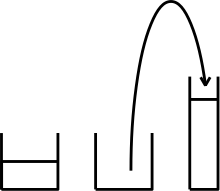
\includegraphics[width=7.5cm]{./images/papert-1/220px-Fig-2-mindstorms.png}
   \label{Papert}
\end{figure}

Per un adulto è ovvio che versando liquido da un bicchiere ad un altro il volume del liquido non cambia (a meno di piccoli effetti, come gocce versate fuori o lasciate nel bicchiere precedente). La conservazione del volume è così ovvia che sembra non sia venuto in mente a nessuno prima di Piaget che ai bambini di quattro anni potrebbe apparire diversamente. Occorre una sostanziale crescita intellettuale prima che i bambini sviluppino una visione “conservazionista” del mondo. La conservazione del volume è solo una delle tante conservazioni che devono imparare.  Un'altra è la conservazione dei numeri. Anche in questo caso, gli adulti faticano a rendersi conto che un bambino   deve imparare il fatto che contando una collezione di oggetti in ordine diverso il risultato sia lo stesso. Per gli adulti l'operazione di contare significa semplicemente determinare quanti oggetti “ci sono”. Il risultato dell'operazione è un “fatto oggettivo” indipendente dall'atto di contare. Ma la separazione del numero dal conteggio (del prodotto dal processo) poggia su presupposti epistemologici che sono non solo ignoti al bambino preconservazionista, ma anche estranei alla loro visione del mondo. Tali conservazioni rappresentano solo una parte della vasta struttura di conoscenza matematica nascosta che i bambini imparano da soli. Nella geometria intuitiva del bambino di quattro o cinque anni, la linea retta non è necessariamente la distanza più breve fra due punti, e che camminare lentamente fra due punti non richiede necessariamente più tempo che camminare velocemente. Anche in questo caso, non è che manchi semplicemente un elemento di conoscenza, bensì il presupposto che sostiene l'idea “del più breve” quale proprietà di un percorso piuttosto che dell'azione di percorrerlo. 

Nessuno di questi casi deve essere interpretato come una carenza di conoscenza da parte del bambino. Piaget ha mostrato come i bambini piccoli abbiano teorie del mondo che, nei propri termini, sono perfettamente coerenti. Queste teorie sviluppate spontaneamente da tutti i bambini, hanno componenti ben sviluppati che non sono meno “matematici”, sebbene esprimano una matematica diversa, rispetto a quella accettata dalla nostra cultura (adulta). Il processo di apprendimento nascosto ha due fasi: già in età prescolare ogni bambino sviluppa teorizzazioni proprie del mondo per poi spostarsi verso visioni caratteristiche dell'età adulta. E questo accade attraverso quello che ho chiamato apprendimento piagetiano, un processo con caratteristiche che la scuola dovrebbe invidiare: funziona (accade in tutti i bambini), è economico (non richiede maestri ne curricula), e è “umano” (i bambini lo attuano con spirito apparentemente disinteressato senza bisogno di riconoscimenti o punizioni esplicite imposti dall'esterno).  

La misura in cui nella nostra società gli adulti hanno perso l'atteggiamento positivo dei bambini nei confronti dell'apprendimento varia da individuo a individuo. Una quota sconosciuta ma certamente significativa della popolazione ha completamente rinunciato a imparare. Queste persone raramente, se non mai, si cimentano nell'apprendimento e non si sentono né competenti né capaci di trarne giovamento. Il costo personale e sociale è enorme: la matofobia può limitare la vita delle persone, culturalmente e materialmente. Un numero ancora maggiore di persone non ha rinunciato completamente ma soffre di pesanti limitazioni a causa di pregiudizi negativi profondamente radicati sulle proprie capacità. La deficienza diventa identità: “Io non posso imparare il francese, non ho orecchio per le lingue;” “Non potrei mai fare affari, non ho la testa per i numeri.” “Non posso imparare lo sci parallelo, non sono mai stato coordinato.” Queste credenze sono spesso manifestate ripetutamente, in modo rituale, come superstizioni. E, come le superstizioni, creano un mondo di tabù; in questo caso il tabù dell'apprendimento. In questo capitolo e nel capitolo 3, discuteremo su degli esperimenti che dimostrano come queste immagini di se spesso corrispondano a una realtà molto limitata – usualmente la “realtà scolastica” di una persona. In un contesto formativo, con un adeguato supporto emozionale e intellettuale, lo “scoordinato” può imparare esercizi circensi come la giocoleria e coloro che “non hanno la testa per i numeri” possono scoprire che non solo sono in grado di capire la matematica ma vi si possono anche appassionare.

Sebbene tali opinioni negative su di se possano essere superate, di fatto sono estremamente tenaci e tendono ad autoconfermarsi. Se uno crede abbastanza fermamente di non poter fare matematica, avrà quasi sicuramente successo nell'impedirsi di fare qualsiasi cosa che gli paia attinente alla matematica. La conseguenza di tale autosabotaggio è il fallimento personale, e ogni fallimento rinforza l'assunto di base. Ancora più insidiosi sono i pregiudizi che appartengono non solo agli individui ma a un'intera cultura.

I nostri figli crescono in una cultura permeata dall'idea che ci siano “persone brillanti” e “persone stupide”. La costruzione sociale di un individuo è costituita da un fascio di attitudini. Ci sono persone “buone per la matematica”  e persone “negate per la matematica”. Tutto è aggiustato in maniera da attribuire i primi insuccessi o esperienze negative dei bambini a loro proprie disabilità. Di conseguenza, i bambini interpretano i fallimenti come sentenze di appartenenza al gruppo delle “persone stupide” o, più spesso, al gruppo delle persone “inadatte per l'attività x” (dove, come abbiamo osservato, spesso x si identifica con la matematica). In un contesto del genere i bambini declinano la propria personalità nei termini delle loro limitazioni, che verranno confermate e consolidate nel corso degli anni. Solo raramente accade che un evento eccezionale induca qualcuno a riorganizzare la propria immagine intellettuale in modo da aprire nuove prospettive su ciò che può apprendere.

Non è facile rimuovere questi pregiudizi sulla natura delle capacità umane. I pregiudizi popolari sono sempre difficili da sradicare. Ma qui le difficoltà sono sostenute da vari altri fattori. In primo luogo, le teorie comuni sulle attitudini umane sembrano essere sostenute da teorie “scientifiche”. Dopotutto, la psicologia si avvale molto di misure attitudinali. Proviamo a mettere in discussione la significatività di ciò che viene misurato mediante l'esperimento mentale di immaginare una \textit{Mathland}. 

Sebbene l'esperimento mentale lasci aperta la questione di come realizzarla una \textit{Mathland}, questo è tuttavia completamente rigoroso nel dimostrare che i pregiudizi comuni sulle capacità matematiche non sono sostenuti da evidenze palesi. Ma siccome i lettori più matofobici potrebbero avere problemi a fare l'esperimento per conto loro, lo riformulo in un altro modo. Immaginiamo di far disegnare ai bambini per un'ora al giorno passi di danza sulla carta e di far sostenere loro un esame su tali “questioni di danza” prima di lasciarli ballare veramente. Non dovremmo in tal caso aspettarci un mondo pieno di “danzofobi”? E non concluderemmo che coloro che ce la fanno a raggiungere la sala da ballo sono i più dotati per la danza? Io credo che sia altrettanto ingiustificato trarre conclusioni  sulle doti matematiche in base allo scarso entusiasmo dei bambini per passare centinaia di ore a fare somme.

Uno può sperare che passando dalle storie ai metodi più rigorosi della psicologia potremmo ottenere dati più consistenti sulle potenzialità degli individui in termini di competenze raggiungibili. Ma non è così: il paradigma corrente nella psicologia della formazione è focalizzato su come i bambini imparano o (più frequentemente) non imparano la matematica nella “anti-\textit{Mathland}” in cui viviamo. Un indirizzo che può essere descritto da questa storia:

\begin{quote}
Immaginiamo una persona del diciannovesimo secolo che volesse migliorare i sistemi di trasporto. Essa sarebbe stata probabilmente persuasa del fatto che la strada per escogitare nuovi metodi passi dalla conoscenza profonda dei metodi esistenti. Sarebbe così partita con uno studio accurato delle differenze fra i vari tipi di carri trainati da cavalli. Avrebbe quindi documentato accuratamente la dipendenza delle velocità ottenibili in funzione della forma e dei materiali degli assi, dei perni e delle finiture.
\end{quote}

Retrospettivamente sappiamo che la strada dell'evoluzione dei mezzi di trasporto è stata completamente diversa. Le invenzioni dell'automobile e dell'aeroplano non hanno preso le mosse dallo studio dettagliato su come i mezzi preesistenti, ovvero i carri trainati da animali, funzionassero o meno.  Ecco, questo è il  modello della ricerca attuale sulle questioni di formazione. I paradigmi usuali per tale tipo di ricerca pongono al centro degli  studi  la classe scolastica. Ci sono molti studi sullo scarso valore dell'insegnamento che viene impartito dalla scuola nella matematica e nelle scienze. È tuttavia diffusa l'idea che un “buon” approccio pedagogico debba basarsi su questi metodi, in realtà poveri di pensiero. Si può simpatizzare con le buone intenzioni, tuttavia penso che tali strategie riflettano il desiderio di mantenere il sistema tradizionale. Come dire di ritenere che convenga migliorare gli assi dei carri a trazione animale. Invece la questione importante sarebbe quella di inventare l'“automobile della formazione”. Questo problema (tema centrale di questo libro) non viene di fatto affrontato e, di conseguenza, ci sembra che le basi scientifiche che sostengono le assunzioni comuni sulle attitudini siano piuttosto labili. Assunzioni che tuttavia sono istituzionalizzate nelle scuole, nei sistemi di valutazione e di ammissione nelle università, al punto che la loro radicazione sociale è tanto forte quanto deboli sono i presupposti scientifici. 

Dalla scuola dell'infanzia in poi, i bambini sono sottoposti a prove basate su capacità verbali e quantitative concepite come entità “vere” e separabili. I risultati di tali test si trasformano in un corredo di attitudini che determinano la costruzione sociale del bambino. Una volta che Johnny e il suo maestro condividono la percezione che Johnny è una persona dotata per l'arte ma non per la matematica, tale percezione tende inevitabilmente a rinforzarsi con il tempo. Questo è un fatto largamente accettato nella psicologia della formazione. Ma il modo in cui la scuola forma le attitudini presenta aspetti più profondi. Consideriamo il caso di un bambino  che ho seguito durante i suoi ottavo e nono anni di età. Jim era un bambino molto loquace ma matofobico appartenente ad una famiglia di professionisti. La sua passione per le parole e il piacere di parlare si erano manifestate molto prima di andare a scuola. La matofobia era invece comparsa a scuola. La mia teoria è che essa sia stata una diretta conseguenza della sua precocità verbale. Dai genitori avevo appreso che Jim aveva presto sviluppato l'abitudine di commentare a voce alta qualsiasi cosa facesse. Un'abitudine che non aveva causato particolari problemi con i genitori o presso la scuola dell'infanzia. I problemi sono sorti affrontando l'aritmetica. A quel punto aveva già imparato a tenere sotto controllo la sua abitudine ma io sospetto che lui non avesse cessato di commentare le proprie azioni, seppur interiormente. Durante le ore di matematica si trovava in imbarazzo: semplicemente non riusciva a commentare l'attività di fare somme. Gli mancava il vocabolario (come manca alla maggior parte di noi) e non vedeva la motivazione. Questa frustrazione si tramutò in odio per la matematica, la conseguenza del quale fu una valutazione di scarsa attitudine per la materia. 

Per me fu una storia commovente. Credo che molto spesso quella che appare una debolezza intellettuale sia espressione, come nel caso di Jim, di quella che in realtà è una particolare capacità. È non è solo la capacità verbale, chiunque osservi con attenzione i bambini nota processi simili: per esempio un bambino che prediliga l'ordine logico può avere problemi con la sillabazione dell'inglese e magari finire col detestare la scrittura. L'idea di \textit{Mathland} ci suggerisce come il computer potrebbe servire ad evitare i problemi riscontrati da Jim e il suo pari dislessico. Ambedue i bambini sono vittime della netta separazione fra cultura verbale e matematica. Nella \textit{Mathland} che descriviamo in questo capitolo, la passione e la competenza verbale di Jim potrebbero essere mobilizzate per favorire lo sviluppo formale matematico, invece di ostacolarlo, e la passione dell'altro bambino per la logica potrebbe essere sfruttata per sviluppare le sue competenze linguistiche. 

Il concetto di mobilizzare tutte le capacità di un bambino per qualsiasi dominio di attività intellettuale risponde all'idea che attitudini differenti possano riflettere differenze nello sviluppo del cervello. È diventato comune ragionare come se ci fossero diversi cervelli, o diversi “organi” nel cervello. Per la matematica e per la lingua. In accordo con questo pensiero i bambini si dividono fra dotati per attività verbali o matematiche a seconda di quale loro organo cerebrale sia più forte. Ma una simile visione anatomica delle funzioni cerebrali comporta delle assunzioni epistemologiche. Per esempio si assume che si possa accedere alla matematica tramite una sola via e che se questa è “bloccata anatomicamente” allora il bambino non vi potrà accedere. Ora, di fatto, per la maggior parte dei bambini delle società contemporanee la via verso la matematica “avanzata” è una sola e questa è la via della matematica scolastica. Ma anche se ulteriori ricerche nella biologia del cervello arrivassero a dimostrare che tale via dipenda da un organo cerebrale  mancante in alcuni bambini, ciò non significa che la matematica stessa dipenda da organi del genere. Piuttosto, significherebbe che dovremmo cercare altre strade. La tesi sostenuta in questo libro è che esistano altre vie, e che la dipendenza delle funzioni dal cervello sia essa stessa un costrutto sociale

Supponiamo che esista una parte del cervello specializzata nelle manipolazioni mentali dei numeri che insegniamo scuola, e chiamiamola MAD, “\textit{Math Acquisition Device}”\footnote{[NdR] Qui Papert gioca con l'idea del linguista Noam Chomsky, secondo la quale il nostro cervello disporrebbe di una sorta di dispositivo di acquisizione del linguaggio (LAD: \textit{Language} \textit{Acquisition} \textit{Device}). Papert precisa di non credere a tale ipotesi, ritenendo un ipotetico MAD altrettanto improbabile di un LAD. Secondo l'ipotesi di Chomsky il cervello sarebbe composto da un insieme di organi neurologici specializzati per specifiche funzioni intellettuali. Secondo Papert tale ipotesi è troppo grossolana e se, probabilmente, si può ritenere che nel cervello vi siano dei dispositivi specializzati, è semplicistico immaginare che ve ne siano di così complessi da assolvere a funzioni quali il pensiero matematico e verbale.}. In tal caso nel corso dell'evoluzione umana si sarebbero sviluppati metodi per fare e insegnare l'aritmetica in grado di trarre massimo vantaggio dalle proprietà del MAD. Ma se questi metodi funzionassero solo per una parte di noi, e per la società nel suo insieme, si rivelerebbero invece catastrofici per un individuo il cui MAD fosse danneggiato o inaccessibile per qualche altro motivo (magari di origine “neurotica”). Una tale persona fallirebbe a scuola e le verrebbe diagnostica una “discalculia”. E finché noi insistiamo con l'insegnare l'aritmetica ai bambini nel modo convenzionale, continueremo a “dimostrare” tramite i test obiettivi che questi bambini non  possono “fare aritmetica”. Ma questo è come dimostrare che un bambino sordo non possa disporre di un linguaggio perché non sente. Così come la lingua dei segni impiega le mani e gli occhi per aggirare gli organi della parola, così si potrebbero individuare modi alternativi di fare matematica per aggirare il MAD, forse altrettanto validi anche se diversi. 

Ma non c'è bisogno di invocare la neurologia per spiegare come mai alcuni bambini non acquistano confidenza con la matematica. L'analogia con le lezioni di danza senza musica e senza sala da ballo è seria. La nostra cultura della formazione offre poche possibilità agli allievi di matematica per capire veramente ciò che studiano. Di conseguenza i nostri bambini sono forzati a seguire un modello di studio della matematica che è veramente il peggiore. È il modello dell'apprendimento mnemonico, dove i contenuti sono trattati come fossero privi di significato; è un modello “dissociato”. Alcune delle nostre difficoltà nell'insegnamento di una matematica culturalmente più integrabile sono dovute a un problema oggettivo: prima che esistessero i computer c'erano veramente pochi punti di contatto fra i fatti più importanti e coinvolgenti della matematica e l'esperienza quotidiana. Ma il computer – un'entità capace di parlare la matematica presente in modo ubiquitario nella vita di tutti i giorni a casa, nella scuola e al lavoro – può provvedere a tale collegamento. La sfida della formazione è quella di trovare i modi per sfruttare queste tecnologie.

La matematica non è certamente l'unico esempio di apprendimento dissociato. Ma è un ottimo esempio precisamente per il fatto che molti lettori preferirebbero che ora parlassimo d'altro. La nostra cultura è talmente  matofobica che se fosse possibile dimostrare come il computer potrebbe migliorare la nostra relazione con la matematica, avrei fondati motivi per sostenere che si potrebbero migliorare allo stesso modo le relazioni con altri tipi di apprendimento. Le esperienze in \textit{Mathland}, come quella di sostenere una “conversazione matematica”, fanno vivere all'individuo un senso liberatorio delle possibilità di fare una serie di cose che prima sembravano “troppo difficili”. In questo senso il contatto con il computer può aprire l'accesso alla conoscenza, non tanto in senso strumentale per disporre di informazioni processate, ma per porre in discussione alcune assunzioni vincolanti che le persone fanno su di se. La \textit{Mathland} del computer che propongo estende l'apprendimento naturale di tipo piagetiano dell'apprendimento della lingua madre all'apprendimento della matematica. L'apprendimento piagetiano è profondamente radicato in altri tipi di attività. Per esempio, i bambini piccoli non hanno momenti dedicati a “apprendere la lingua”.  Questo è un modello che si pone in contrapposizione all'apprendimento dissociato, che ha luogo in maniera relativamente separata da altre attività, mentali e fisiche. Nella nostra cultura, l'insegnamento della matematica a scuola è paradigmatico dell'apprendimento dissociato . Per la maggior parte della gente la matematica è insegnata e recepita come una medicina. La dissociazione matematica della nostra cultura è quasi una caricatura delle peggiori forme di alienazione epistemologica. Nell'ambiente LOGO si ammorbidiscono le distinzioni: nessuna attività in particolare è connotata a parte come “apprendere la matematica”. Il problema di rendere la matematica comprensibile concerne il problema più generale di rendere comprensibile un linguaggio basato su “descrizioni formali”. Così, prima di passare a esempi di come con il computer si possa provare a dare senso alla matematica, consideriamo alcuni esempi per rendere comprensibili linguaggi basati su descrizioni formali in domini della conoscenza che la gente non associa usualmente alla matematica. Nel primo esempio il dominio è quello della grammatica, per molti temibile quasi quanto la matematica.

Nel corso di uno studio di un anno, in una classe II di scuola  media di I grado di livello medio, una delle attività era quella che gli studenti chiamavano “\textit{computer} \textit{poetry}”. L'attività consisteva nell'usare il computer per comporre frasi: loro inserivano una struttura sintattica che il computer popolava di parole in maniera casuale. Il risultato è una sorta di poesia concreta tipo quella illustrata qui sotto\footnote{[NdR] Abbiamo lasciato la versione originale, ci pare inutile “tradurre” un pezzo simile, ai fini della comprensione del concetto.}:

\begin{quote}
INSANE RETARD MAKES BECAUSE SWEET SNOOPY SCREAMS\\
SEXY GIRL LOVES THATS WHY THE SEXY LADY HATES\\
UGLY MAN LOVES BECAUSE UGLY DOG HATES\\
MAD WOLF HATES BECAUSE INSANE WOLF SKIPS\\
SEXY RETARD SCREAMS THATS WHY THE SEXY RETARD\\
THIN SNOOPY RUNS BECAUSE FAT WOLF HOPS\\
SWEET FOGINY SKIPS A FAT LADY RUNS\\
\end{quote}

Un'allieva di tredici anni, Jenny, aveva commosso lo staff del progetto chiedendo il primo giorno: “Perché avete scelto noi? Noi non siamo i cervelloni. (“\textit{Why were we chosen for this? We're not the brains.}”. Lo studio prevedeva proprio di lavorare con una classe di livello “medio”. Un giorno Jenny entrò tutta eccitata. Aveva fatto una scoperta: “Ora ho capito perché ci  sono i sostantivi e i verbi.” Già da vari anni Jenny aveva fatto esercizi grammaticali, ma non aveva mai capito le differenze fra sostantivi, verbi e avverbi. Ma ora era chiaro che le sue difficoltà non dipendevano dall'incapacità di lavorare con categorie logiche. Il problema era un altro. Lei non aveva semplicemente compreso la finalità della fatica. Non era stata in grado di afferrare il senso della grammatica perché non vedeva a cosa servisse. E quando aveva chiesto a cosa serviva, la spiegazione dell'insegnante le era parsa manifestamente disonesta: “La grammatica ti serve a parlare meglio.”

Infatti, per recuperare la connessione fra l'apprendimento della grammatica e il miglioramento della lingua parlata occorre una visione più ampia del complesso procedimento di apprendimento di una lingua, che Jenny non poteva avere all'età in cui era entrata in contatto con la grammatica. Certamente lei non poteva vedere in che modo la grammatica potesse aiutarla a parlare meglio, né pensava di avere necessità di essere aiutata. Di conseguenza aveva sviluppato un sentimento di rancore per la grammatica. E, come succede alla maggior parte di noi, il rancore garantisce fallimento. Ma quando si è trovata nella condizione di far comporre frasi al computer, è successo qualcosa di interessante, trovandosi nella condizione di dover classificare le parole in categorie non perché qualcuno le avesse chiesto di farlo ma perché ne aveva bisogno. Per “insegnare” al suo computer come comporre serie di parole in maniera che sembrassero frasi compiute occorreva “insegnargli” a scegliere parole appartenenti alle categorie giuste. Ciò che lei aveva imparato sulla grammatica tramite l'esperienza con una  macchina non aveva niente di meccanico né di routinario. Il suo era stato un apprendimento profondo e significativo. Jenny aveva fatto più che imparare le definizioni per una particolare classe grammaticale. Aveva capito l'idea generale che le parole (come le cose) possono essere collocate in gruppi o insiemi diversi, e che fare questo può essere utile. Non aveva solo “capito” la grammatica ma aveva cambiato il suo atteggiamento nei suoi confronti. Era “sua”, e nel corso dell'anno, altri casi simili l'aiutarono rivedere la propria immagine. Cambiarono anche i suoi risultati; i suoi voti, prima medio-bassi, divennero massimi per il resto degli anni scolastici. Imparò che anche  lei poteva essere “un cervellone”, dopo tutto.

È naturale come matematica e grammatica non vengano capite dai bambini quando non sono capite da chi sta loro intorno e come, affinché la comprendano, occorra qualcosa di più di un insegnante che dica la cosa giusta o disegni il diagramma giusto alla lavagna. Ho chiesto a molti insegnanti e genitori cosa pensassero della matematica e perché fosse importante impararla. Pochi di loro hanno espresso una visione sufficientemente coerente da giustificare l'impiego di varie migliaia di ore della vita di un bambino per impararla, e questo i bambini lo sentono. Quando un insegnante spiega a uno studente che tutte quelle ore di aritmetica servono a essere in grado di controllare il resto al supermercato, questo non viene semplicemente creduto. I bambini interpretano tali “motivazioni” come un ulteriore esempio di malafede da parte degli adulti. Lo stesso effetto si manifesta dicendo ai bambini che la matematica scolastica è “divertente”, quando è loro chiaro che gli insegnanti che si esprimono così per divertirsi fanno tutt'altre cose. Ne aiuta molto spiegare che la matematica serve per diventare scienziati poiché la maggior parte di loro non prevede una cosa del genere.  La maggior parte dei bambini si rende conto che l'insegnante non ama la matematica più di quanto la amino loro e che la ragione per cui va fatta è semplicemente perché lo prevede il curricolo. Tutto ciò erode la fiducia dei bambini nel mondo degli adulti e nel processo di educazione. \textit{E io penso che introduca un elemento di profonda disonestà nella relazione educativa}\footnote{[NdR] Corsivo dell'autore.}.

I bambini percepiscono la retorica scolastica sulla matematica come un discorso in malafede. Al fine di rimediare la situazione dobbiamo prima riconoscere che la percezione dei  bambini è sostanzialmente corretta. Il “tipo di matematica” rifilata nelle scuole non è né significativa, né divertente e nemmeno utile. Ciò non significa che alcuni bambini non la possano vivere come un gioco personale importante e piacevole. Alcuni lo fanno per i voti; altri per barcamenarsi con l'insegnante e il sistema. Per molti, la matematica scolastica è piacevole proprio nella sua ripetitività, esattamente perché priva di significato e dissociata così da costituire un riparo da dover comprendere cosa stia accadendo in classe. Ma tutto questo mostra l'ingenuità dei bambini. Non si può giustificare la matematica scolastica sostenendo che, malgrado la sua intrinseca opacità, i bambini creativi vi trovino senso e divertimento.

È importante ricordarsi la distinzione fra matematica – un vasto dominio di indagine la cui bellezza è raramente immaginata da chi non è un matematico – e qualcos'altro che chiamerò “matematica scolastica”. 

Io interpreto la matematica scolastica come una costruzione sociale, una specie di QWERTY\footnote{[NdR] QWERTY denota la disposizione usuale delle tastiere, dalla prima linea di tasti in alto, leggendoli da sinistra verso destra. Papert in un'altra parte del libro (Cap. 1 – I computer e le culture del computer, pag. 32-34) descrive come tale disposizione si sia stabilita con le prime macchine da scrivere meccaniche, quando i tasti avevano una certa tendenza ad incepparsi. Per tale motivo prevalse empiricamente una disposizione che minimizzasse la battitura consequenziale di tasti adiacenti, circostanza che favoriva l'inceppamento. Ben presto l'evoluzione tecnica rese inutile tale accorgimento ma la disposizione QWERTY era ormai consolidata e sarebbe ormai stato antieconomico cambiare tutto il sistema, con una moltitudine di macchine a giro per il mondo è una competenza dattilografica ormai assestata su quello standard. Papert nota come universalmente si ritenga tale disposizione ottimale, sebbene non vi siano giustificazioni tecniche concrete a parte la motivazione iniziale ormai desueta, e utilizza, anche nel proseguio del libro, il “fenomeno QWERTY per connotare altri “intrappolamenti” del pensiero che vengono giustificati a posteriori con argomenti tecnici artificiosi quando invece le vere motivazioni consistono unicamente in varie forme di inerzia.}. Un insieme di accidenti storici (che discuteremo in breve) ha determinato la scelta degli argomenti matematici che dovrebbero costituire il bagaglio matematico di un cittadino. Come nel caso della disposizione QWERTY  dei tasti, la matematica scolastica ha avuto qualche senso in un certo contesto storico. Ma, analogamente, si è radicata così bene che tutti la danno per scontata, costruendo razionalizzazioni  per giustificarla, ben dopo la scomparsa delle condizioni storiche che l'avevano generata. Effettivamente, per la maggior parte della gente nella nostra cultura è inconcepibile che la matematica scolastica possa essere differente: questa è l'unica matematica che conoscono. Per tentare di rompere questo circolo vizioso, condurrò il lettore in un nuovo territorio matematico, la geometria della Tartaruga\footnote{[NrR] \textit{Turtle} \textit{geometry}.}, che con i miei colleghi abbiamo creato per dare ai bambini una prima introduzione più significativa al mondo della matematica formale. I criteri di progetto della geometria della Tartaruga si comprendono meglio esaminando più da vicino le circostanze storiche che hanno formato la matematica scolastica.

Alcune di queste circostanze erano pragmatiche. Prima che comparissero le calcolatrici elettroniche,   era una concreta necessità sociale quella di “programmare” molte persone affinché fossero in gradi di fare velocemente e accuratamente operazioni come lunghe divisioni. Ma ora che le calcolatrici sono accessibili economicamente dovremmo  riconsiderare l'utilità di dedicare svariate centinaia di ore della vita di ciascun bambino a imparare operazioni del genere. Non intendo negare il valore intellettuale di certa conoscenza, di molta conoscenza veramente, intorno ai numeri. Ben lungi da ciò. Ma possiamo selezionare questa conoscenza in base a criteri coerenti e razionali. Ci possiamo liberare dalla tirannia di considerazioni superficiali e pragmatiche che avevano determinato le scelte del passato su cosa debba essere imparato e a quale età.

Ma l'utilità era solo una delle motivazioni storiche per la matematica scolastica; altre erano di natura \textit{matetica}\footnote{[NdR] Corsivo dell'autore. Devoto Oli: Matetico. Nelle scienze e tecniche dell'educazione, che riguarda l'apprendimento, formativo: \textit{mezzi audiovisivi a scopo m.} [Dal gr. \textit{Máthēsis} 'apprendimento', per influsso dell'ingl. \textit{mathetic}].}. La matetica è l'insieme di principi guida che governano l'apprendimento. Alcune delle motivazioni storiche della matematica scolastica concernevano quello che poteva essere imparato e insegnato prima dell'avvento dei computer. Io credo che il fattore predominante che ha determinato quale matematica dovesse comporre la matematica scolastica fosse il contesto della classe scolastica dotata della tecnologia primitiva fatta di carta e matita. Per esempio, uno studente può disegnare un grafico con carta e matita. Così fu deciso di far disegnare molti grafici. Considerazioni simili hanno influenzato l'enfasi su certi tipi di geometria. Per esempio, nella matematica scolastica “geometria analitica” è diventata sinonimo di rappresentazione grafica delle equazioni. Il risultato è che ogni persona istruita si ricorda vagamente che $y = x^2$ rappresenta una parabola. E, sebbene la maggior parte dei genitori non abbia idea della ragione per cui ciò sia importante, questi si indignano se i anche i loro figli non lo imparano. Assumono che debbano esistere una ragione profonda e obiettiva, nota a coloro che conoscono meglio tali questioni. Ironicamente, è la propria matofobia che impedisce alle persone di esaminare tali ragioni più attentamente, trovandosi così alla mercé di sedicenti esperti di matematica. Pochissime  persone sospettano che la ragione per ciò che viene incluso o meno nella matematica scolastica è così banalmente tecnologica come la facilità con cui si disegna una parabola con carta e matita! Questo è quello che può cambiare così profondamente grazie ai computer: la varietà di costrutti matematici facilmente producibili è smisuratamente più ampia.

Un altro fattore matetico nella costruzione sociale della matematica scolastica è la tecnologia della votazione. Una lingua viva si impara parlando e non necessita di un insegnante che verifica e dà voti a ciascuna frase. Una lingua morta richiede invece un “riscontro” costante da parte di un insegnante. L'attività nota come “sommare” realizza un tale riscontro nella matematica scolastica. Questi piccoli esercizi ripetitivi assurdi hanno un solo merito: sono facili da valutare. E questo vantaggio li ha consolidati ben bene al centro della matematica scolastica. In sintesi, io ritengo che l'edificio della matematica scolastica sia fortemente influenzato da ciò che sembrava possibile insegnare quando la matematica veniva somministrata come una materia “morta”, usando tecnologie primitive di  tipo passivo, come sabbia e bastoni, lavagna e gesso, carta e matita. Il risultato è stato un insieme intellettualmente incoerente di argomenti che viola i più elementari  principi matetici in merito a cosa renda certi argomenti facili da imparare e altri quasi impossibili. 

A fronte dello stato di cose nella scuola, la formazione matematica può prendere due strade. Con l'approccio tradizionale la matematica scolastica viene data per scontata e ci si ingegna di insegnarla in qualche modo. Taluni usano i computer, ma, paradossalmente, l'impiego più comune è quello di impippiare materiale indigeribile, residuato dall'epoca pre-computer. Nella geometria della Tartaruga  il computer è usato in modo totalmente differente, come un mezzo matematicamente espressivo, che ci libera dalla necessità di individuare argomenti matematici possibili da imparare, significativi e intellettualmente coerenti. Invece di porre la questione di come insegnare la matematica scolastica esistente, poniamo quella di “ricostruire la matematica”, o più generalmente, di ricostruire la conoscenza in maniera che non debba essere così difficile insegnarla. 

Ogni “revisione del curriculum” potrebbe essere riformulata in termini di “ricostruzione della conoscenza”. Per esempio, con la riforma del curriculum \textit{New Math}\footnote{[NdR] Questo è palesemente un riferimento storico, da riferire all'epoca e da contestualizzare nella realtà americana.} degli anni Sessanta, qualche tentativo di cambiare i contenuti della matematica scolastica è stato fatto, ma non è cambiato molto. Le somme sono rimaste, anche se riformulate in modo un po' diverso. Il fatto che  le nuove somme si riferissero agli insiemi anziché ai numeri, o all'aritmetica in base 2 anziché in base 10 ha cambiato poco. Inoltre, la riforma della matematica scolastica non ha introdotto nessuna sfida attinente alla creatività dei matematici, non presentando così nessuna delle scintille che caratterizzano la formazione di pensiero nuovo. La denominazione stessa – \textit{New} \textit{Math} – si è rivelata impropria. C'era veramente poco di nuovo nei contenuti: niente di attinente a un processo di invenzione della matematica dei bambini, piuttosto ad una banalizzazione della matematica dei matematici. I bambini meritano qualcosa di meglio di una selezione di vecchia matematica. Come i vestiti passati dai fratelli maggiori, che non tornano mai bene. 

La geometria della Tartaruga ha presso le mosse con l'obiettivo di adattarsi ai bambini. Il primo criterio è quello della “appropriabilità”. Naturalmente i contenuti matematici devono essere pregnanti, ma vedremo che appropriabilità e pensiero matematico serio non sono affatto incompatibili. Al contrario: ci accorgeremo che alcune di tali personali conoscenze acquisite sono le più profondamente matematiche. In vari modi la matematica – per esempio la matematica dello spazio e del movimento, gli schemi ripetitivi delle azioni – è ciò che viene più naturale ai bambini. Lavorando insieme ai miei colleghi su queste idee, sono emersi alcuni concetti in grado di conferire più struttura al concetto di matematica appropriabile. In primo luogo, il principio di continuità: la matematica proposta deve essere in continuità con altre conoscenze, dalle quali possa ereditare un senso di familiarità e valore, insieme a competenza “cognitiva”. Poi il “principio di potenza”: dare allo studente il potere di affrontare progetti personali significativi, altrimenti impossibili. Infine il principio della “risonanza culturale”: gli argomenti devono avere senso in un contesto sociale allargato. Abbiamo parlato della geometria della Tartaruga che risulti comprensibile per i bambini. Ma questo non avverrà se non viene accettata anche dagli adulti. Una matematica di valore non può essere qualcosa che ci permettiamo di infliggere come fosse una medicina amara, e che non vediamo motivo di somministrare a noi stessi.












